\documentclass[tikz,border=10pt]{standalone}
\usepackage{tikz}
\usetikzlibrary{positioning, arrows.meta}
\usetikzlibrary{calc}

\begin{document}

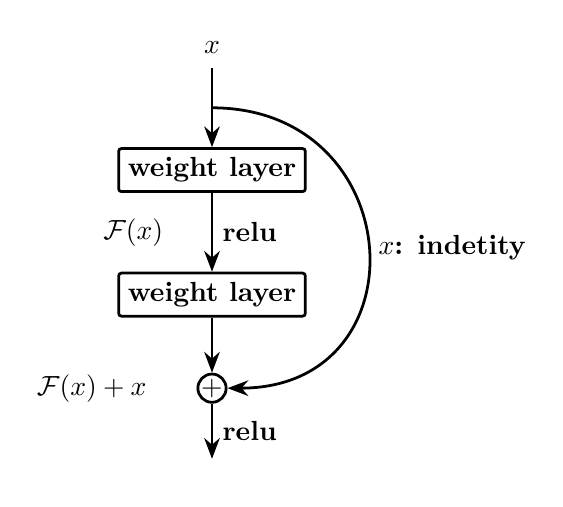
\begin{tikzpicture}[>=Stealth, 
    node distance=1cm,
    every node/.style={font=\bfseries}, % Make all text bold
    every path/.style={line width=1pt}, % Make all lines bold]
]
% Input node
\node (input) [minimum width=1.5cm, minimum height=0.5cm] {$x$};

\node (w1) [draw, rectangle, minimum width=1.5cm, minimum height=0.5cm,rounded corners=1pt,below=of input] {weight layer};
\node (w2) [draw, rectangle, minimum width=1.5cm, minimum height=0.5cm, rounded corners=1pt,below=of w1] {weight layer};

% Add and equals nodes
\node (add) [circle, draw, inner sep=0pt, minimum size=0.25cm, below=0.7cm of w2] {$+$};
\node (invisible) [below=0.7cm of add] {};

% Connection arrows
\draw[->] (input) -- (w1);
\draw[->] (w1) -- node[right] {relu} (w2);
\node (denotation) at ($(w1)!0.5!(w2) + (180:1cm)$) {$\mathcal{F}(x)$};

% \draw[->] (input) -- ++(0, -1.5cm) -| (add);
\draw[->, out=0, in=0, looseness=1.8] (input.south) ++(0, -0.5cm) to node[right] {$x$: indetity} (add);
\draw[->] (w2) -- (add);
\node (con) [left=0.5cm of add] {$\mathcal{F}(x) + x$};
\draw[->] (add) -- node[right]{relu} (invisible);

\end{tikzpicture}

\end{document}

